\documentclass[Main]{subfiles}
\begin{document}

\lstset{language=Matlab,%
    basicstyle=\ttfamily,%
    breaklines=true,%
    morekeywords={matlab2tikz},
    keywordstyle=\color{blue},%
    morekeywords=[2]{1}, keywordstyle=[2]{\color{black}},
    identifierstyle=\color{black},%
    stringstyle=\color{mylilas},
    commentstyle=\color{mygreen},%
    showstringspaces=false,%without this there will be a symbol in the places where there is a space
   % numbers=left,%
   % numberstyle={\tiny \color{black}},% size of the numbers
    %numbersep=9pt, % this defines how far the numbers are from the text
    emph=[1]{for,end,break},emphstyle=[1]\color{red}, %some words to emphasise
    %emph=[2]{word1,word2}, emphstyle=[2]{style},    
}


\chapter{Decoder}

This chapter describes the Meggitt decoder, and the MATLAB implementation created during this project.

\section{Operation of the Meggitt decoder} \label{sec:MeggitOperation}

When decoding cyclic codes, the straight forward approach involves creating a table, that matches all possible error patterns to the corresponding syndrome vector. This approach is impractical when creating a decoding circuit, because the complexity of the circuit tends to grow exponentially with code length and number of errors corrected \cite{lec7}.

This problem can be remedied using the Meggitt decoder. The basis of the Meggitt decoder is Theorem 3.1 presented during lecture 7\cite{lec7}.

\noindent
\framebox{\parbox{\dimexpr\linewidth-2\fboxsep-2\fboxrule}{
 \textbf{Theorem 3.1:} If the received polynomial
$r (x) = r_0 + r_1X + r_2X^2 ... + r_{n-1} X^{n-1}$  generates the syndrome
polynomial $S(X)$. Then a cyclic right shift of the received polynomial $r^{(1)}(X)$ generates the syndrome polynomial $S^{(1)}(X)$. $S^{(1)}(X)$ is actually the remainder of dividing $XS(X)$ by generator polynomial $g(X)$.
}}

Theorem 3.1 can be summarized as such:

\begin{center}

$ r(X) \hspace*{2em}  \Rightarrow^{rightshift} \hspace*{2em} r^{(1)}(X)$ \\
$ \Downarrow \hspace*{12em} \Downarrow$ \\
$ S(X) \hspace*{9em} S^{(1)}(X)$ \\
\end{center}

The syndrome vector can be calculated using equation \ref{eq:syndromeEq}.

\begin{equation} \label{eq:syndromeEq}
r(X) = q(X)g(X)+s(X)
\end{equation}

The syndrome calculation in the Meggitt decoder is implemented by the circuit in figure \ref{fig:syndromeCirc}. The received vector $r(X)$ is shifted in one bit at a time. When $r(X)$ has been shifted in, the syndrome vector is contained in the syndrome register ($S_0, S_1, ... ,S_{n-k-1}$).

\begin{figure}[H]
    \centering
    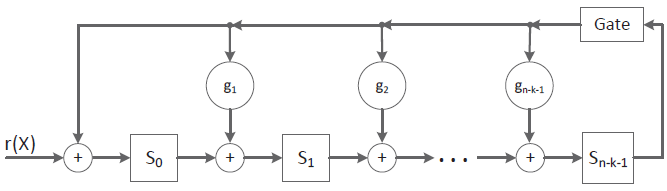
\includegraphics[width=0.8\textwidth]{figures/syndromeCircuit}
    \caption{Syndrome calculating circuit}
    \label{fig:syndromeCirc}
\end{figure}

The entire Meggitt circuit is shown on figure \ref{fig:meggitCirc}. The Meggitt decoder only corrects one bit at a time -- the most significant bit. This simplifies the circuit.

\begin{figure}[H]
    \centering
    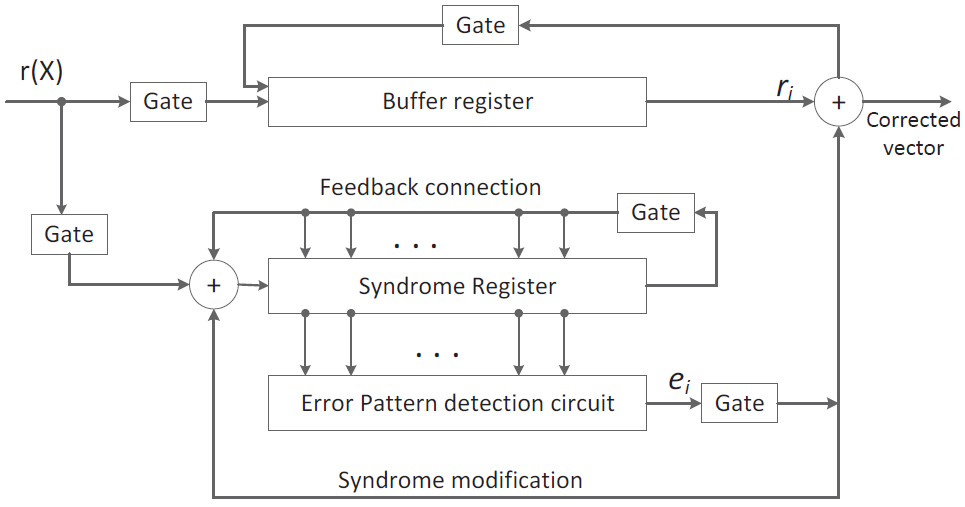
\includegraphics[width=0.8\textwidth]{figures/meggitCircuit}
    \caption{Meggitt circuit}
    \label{fig:meggitCirc}
\end{figure}

The steps taken to perform Meggitt decoding are as follows:

\begin{enumerate}
\item Shift $r(X)$ into the decoder, thus calculating the syndrome vector and populating the buffer with the received vector.
\item \label{enm:loopStart} Check if the syndrome register matches a syndrome vector corresponding with an error pattern with the highest bit in error.
\begin{enumerate}
\item if not the case: shift $r(X)$(the buffer) and $s(X)$.
\item if is the case
\begin{enumerate}
\item Complement MSb of the buffer.
\item Shift the buffer to create $r_1(X)$.
\item Shift the syndrome register to create $S_1^{(1)}(X)$.
\end{enumerate}
\end{enumerate}
\item Repeat the process in \ref{enm:loopStart} for each bit in the received vector $r(X)$.
\end{enumerate}

\section{Decoder implementation overview}\label{sec:decImplOv}

The functionality of the Meggitt decoder is implemented in the file \code{MeggittDecoderImpl.m} which is included in appendix \ref{App:SourceCode}. The Meggitt decoder is implemented in the MATLAB class \code{MeggittDecoderImpl} with UML diagram shown in figure \ref{fig:meggittUML}.

\begin{figure}[h]
    \centering
    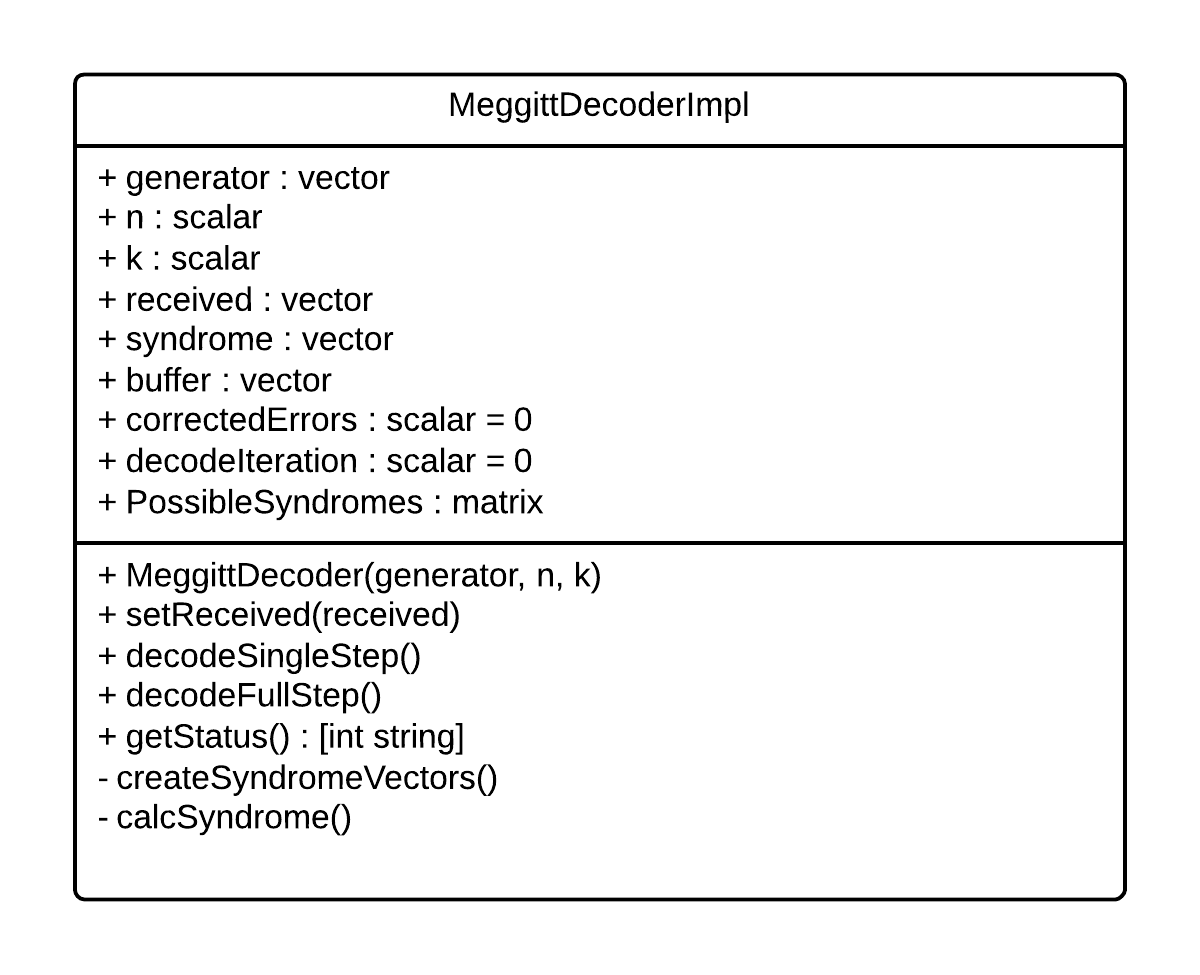
\includegraphics[width=0.7\textwidth]{figures/MeggitDecoderUML}
    \caption{Meggitt decoder UML class diagram}
    \label{fig:meggittUML}
\end{figure}

A sample usage of the decoder class and the encoder function is shown in listing \ref{lst:sample}. The sample uses the generator polynomial stated in the conditions of the project.

\begin{lstlisting}[label={lst:sample},captionpos=b, caption=Sample usage of the decoder.] 
%setup
g = [1 0 0 0 1 0 1 1 1]; %g(x) = 1 + X^4 + X^6 + X^7 + X^8
n = 15;
k = 7;
m = [1 0 1 0 1 0 1];
c = EncodeCyclicSystematic(g, m);
e = [0 0 0 0 0 0 0 0 0 0 0 0 1 0 1];
r = mod(c + e, 2);

md = MeggittDecoderImpl(g, n, k)	%initialize decoder
md.setReceived(r)			%set received vector
md.decodeFullStep()			%perform decoding
decoded = md.buffer;		%buffer contains the decoded vector
eCalc = md.getErrorVector();
\end{lstlisting}

\code{md.decodeFullStep()} runs all or remaining decoding iterations -- a single decoding iteration can be performed using \code{md.decodeSingleStep()}. This allows monitoring of the class data properties such as the buffer and syndrome registers between iterations during the decoding.

\section{Generation of syndrome vectors}
Because the Meggitt decoder only corrects the most significant bit at a given time, the Meggitt decoder only needs to detect syndome vectors, which correspond to an error pattern with the highest bit in error. The function \code{createSyndromeVectors()} generates a matrix, S, containing the relevant syndrome vectors, when an instance of the \code{MeggittDecoderImpl} class is created. The part of the function relevant for a code capable of correcting 2 errors is shown in listing (\ref{lst:CreateSyndromes}). \code{MD} is the instance of the decoder class.

\begin{lstlisting}[label={lst:CreateSyndromes},captionpos=b, caption=Creating possible syndrome vectors.] 
%create 2 bit error patterns with highest bit in error
E = eye(MD.n);
E(:,MD.n) = 1;

H = cyclgen(MD.n,MD.g,'system'); %create parity check matrix
MD.PossibleSyndromes = mod(E*H',2); %calc all syndrome vectors
\end{lstlisting}

\section{Decoder implementation} \label{sec:decoderImpl}
The key part, and also the most difficult part, of the decoder is implementing the algorithm to perform an iteration of the Meggitt decoding process described in section \ref{sec:MeggitOperation}. The function \code{decodeSingleStep()} implements this functionality and is shown in listing \ref{lst:decodeSingleStep}.

\begin{lstlisting}[label={lst:decodeSingleStep},captionpos=b, caption=Decoding a single iteration.] 
%check if the syndrome vector corresponds to an error pattern with 1 as highest bit
if ismember(MD.syndrome, MD.PossibleSyndromes, 'rows') %if PossibleSyndromes contains a vector equal to syndrome
	MD.buffer(end) = mod(MD.buffer(end) + 1, 2); %correct the buffer
	MD.synMod = 1; %syndrome modification
	MD.correctedErrors = MD.correctedErrors + 1;
else
	MD.synMod = 0;
end
  
gate = MD.syndrome(end); %store msb for feedback calc
MD.syndrome = circshift(MD.syndrome,[0 1]); %shift syndrom 1 right
MD.syndrome(1) = 0; %reset lsb to counter circshift() wrapping around
MD.buffer = circshift(MD.buffer,[0 1]); %shift syndrom 1 right    

%calc and apply feedback
feedback = gate * MD.generator;
feedback(end) = []; %remove msb
MD.syndrome = mod(MD.syndrome + feedback, 2); %add feedback to syndrom
MD.syndrome(1) = mod(MD.syndrome(1) + MD.synMod, 2); %apply syndrome modification

MD.decodeIteration = MD.decodeIteration + 1;
\end{lstlisting}

The function \code{decodeFullStep()} performs a full decoding by calling \code{decodeSingleStep()} repeatedly until $n$ iterations have been run.

The initial syndrome vector is calculated by the function  \code{calcSyndrome()} when \code{setRecieved()} is called using a similar algorithm as \code{decodeSingleStep()}.



\end{document} 
